%!TEX encoding = UTF-8 Unicode

%!TEX root = ../compendium2.tex

\Teamlab{\LabWeekNINE}

\begin{Goals}
%!TEX encoding = UTF-8 Unicode
%!TEX root = ../compendium2.tex

\item Kunna använda arv.
\item Kunna göra överskuggning av medlemmar i en supertyp med \code{override}.
\item Kunna referera till medlemmar i superklassen med \code{super} vid överskuggning.
\item Kunna förklara begreppet dynamisk bindning.

\end{Goals}

\begin{Preparations}
\item Gör övning {\tt \ExeWeekNINE} i kapitel \ref{exe:W09}.
%!TEX encoding = UTF-8 Unicode
%!TEX root = compendium.tex
\item 
Diskutera i din samarbetsgrupp hur ni ska dela upp koden mellan er i flera olika delar, som ni kan arbeta med var för sig. En sådan del kan vara en klass, en trait, ett objekt, ett paket, eller en funktion. 
\item
Varje del ska ha en \emph{huvudansvarig} individ. 
\item
Arbetsfördelningen ska vara någorlunda jämnt fördelad mellan gruppmedlemmarna.
\item
När ni redovisar er lösning ska ni börja med att redogöra för handledaren hur ni delat upp koden och vem som är huvudansvarig för vad. 
\item
Den som är huvudansvarig för en viss del redovisar den delen.
\item 
Grupplaborationer görs i huvudsak som hemuppgift. Salstiden används primärt för redovisning.
\item Träffas i din samarbetsgrupp och diskutera ert arbetssätt utifrån följande frågeställningar:
\begin{itemize}
  \item Vilken av era varianter av \code{Turtle} ska ni utgå ifrån?
  \item Hur ska ni jobba med gemensamma koddelar?
  \item Hur ska ni dela med er av de koddelar som ni utvecklar var för sig?
\end{itemize}

\end{Preparations}

\subsection{Bakgrund}

I denna grupplaboration ska ni skapa en sköldpaddstävling med 8 olika instanser av speciella tävlingssköldpaddor, som försöker vinna genom att komma först i mål.

Ni ska skapa en arvshierarki från \code{Turtle}-klassen från tidigare labb, enligt figur~\ref{turtle-race:fig:uml-diagram1}.
Med utgångspunkt från \code{Turtle} ska ni skapa följande subtyper:
\begin{itemize}
  \item En subtyp \code{class ColorTurtle extends Turtle} som har en färg och som överskuggar metoden \code{forward}, så att den valda färgen används när ett spår ritas.
  \item En subtyp \code{class RaceTurtle extends Turtle} som kan ingå i en tävling och som vid anrop av \code{raceStep} tar ett steg med slumpmässig längd. En \code{RaceTurtle} har även andra attribut, t.ex. ett startnummer \code{nbr} och ett namn \code{name} (visas ej i figur~\ref{turtle-race:fig:uml-diagram1}).
\end{itemize}

\noindent Ni ska även skapa minst en subtyp per gruppmedlem till \code{RaceTurtle} som ger tävlingssköldpaddor speciella egenskaper som ni själva väljer.

När ni är klara kan en sköldpaddstävling se ut som i figur~\ref{turtle-race:fig:race}.
Till er hjälp har ni den färdiga klassen \code{RaceWindow} som utvidgar \code{SimpleWindow} med attribut och metoder för att skapa tävlingsbanan, enligt kod på sidan \pageref{turtle-race:RaceWindow}. Metoden \code{draw} ritar ut en tävlingsbana, metoden \code{writeRacerList} skriver ut en lista med deltagare och metoden \code{writeTitle} ger tävlingsbanan en överskrift. Ni får gärna förbättra och förändra utseendet på tävlingsbanan.

\begin{figure}
\begin{center}
\newcommand{\TextBox}[1]{\raisebox{0pt}[1em][0.5em]{#1}}
\tikzstyle{umlclass}=[rectangle, draw=black,  thick, anchor=north, text width=4cm, rectangle split, rectangle split parts = 3]
\begin{tikzpicture}[inner sep=0.5em,scale=1.2, every node/.style={transform shape}]

  \node [umlclass, rectangle split parts = 1, xshift=0cm, yshift=4cm] (BaseType1)  {
              \textit{\textbf{\centerline{\TextBox{\code{Turtle}}}}}
              %\nodepart[]{second}\TextBox{~}
          };


  \node [umlclass, rectangle split parts = 2, xshift=0cm, yshift=2.5cm] (BaseType2)  {
              \textit{\textbf{\centerline{\TextBox{\code{ColorTurtle}}}}}
              \nodepart[]{second}\TextBox{\code{var color: Color}}
          };

\node [umlclass, rectangle split parts = 2, xshift=0cm] (BaseType3)  {
            \textit{\textbf{\centerline{\TextBox{\code{RaceTurtle}}}}}
            \nodepart[]{second}\TextBox{\code{val defaultStep: Int}}
        };

% \node [umlclass, rectangle split parts = 2]  at (5cm,-3cm) (SubType1) {
%             \textbf{\centerline{\TextBox{\code{Dizzy}}}}
%             \nodepart[]{second} \TextBox{\code{val dizziness: Int}}
%         };
%
% \node [umlclass, rectangle split parts = 2]  at (0cm,-3cm) (SubType2) {
%           \textbf{\centerline{\TextBox{\code{AbsentMinded}}}}
%           \nodepart[]{second} \TextBox{\code{val chance: Int}}
%         };
%
% \node [umlclass, rectangle split parts = 2] at (-5cm,-3cm) (SubType3)  {
%             \textbf{\centerline{\TextBox{\code{Mole}}}}
%             \nodepart[]{second} \TextBox{\code{val digging: Double}}
%         };
% \draw[umlarrow] (SubType1.north) -- ++(0,0.5) -| (BaseType3.south);
% \draw[umlarrow] (SubType2.north) -- ++(0,0.5) -| (BaseType3.south);
% \draw[umlarrow] (SubType3.north) -- ++(0,0.5) -| (BaseType3.south);
\draw[umlarrow] (BaseType3.north) -- ++(0,0.5) -| (BaseType2.south);
\draw[umlarrow] (BaseType2.north) -- ++(0,0.5) -| (BaseType1.south);

\end{tikzpicture}
\end{center}
\caption{Arvshierarki med \code{Turtle} som bastyp.}
\label{turtle-race:fig:uml-diagram1}
\end{figure}



\begin{figure}
\centering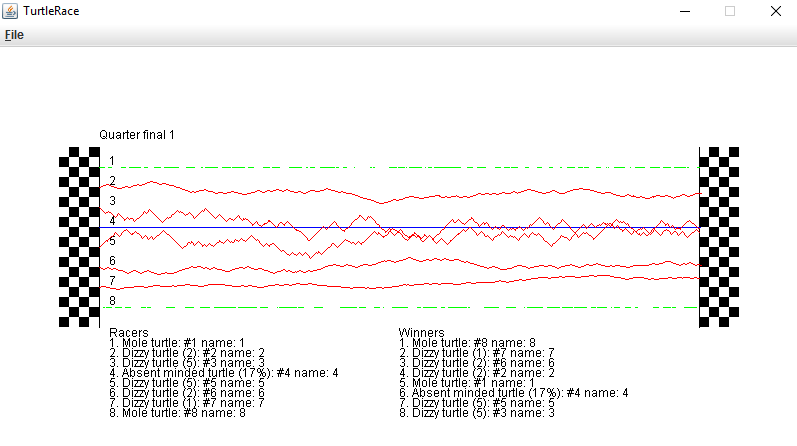
\includegraphics[width=1.02\textwidth, trim={1.5cm 0.2cm 1.5cm 3cm},clip]{../img/turtlerace/RaceWindow}
\caption{Exempel på en sköldpaddstävling i ett \code{RaceWindow}.}
\label{turtle-race:fig:race}
\end{figure}


\begin{figure}
  \scalainputlisting[basicstyle=\ttfamily\fontsize{10}{13}\selectfont]{../workspace/w09_turtlerace_team/src/main/scala/turtlerace/RaceWindow.scala}
  \caption{Den färdiga klassen \code{RaceWindow}.}
  \label{turtle-race:RaceWindow}
\end{figure}


\subsection{Obligatoriska uppgifter}

\Task Gör klart \code{ColorTurtle} enligt nedan. Testa noga så att allt fungerar.

\scalainputlisting[basicstyle=\ttfamily\fontsize{10}{13}\selectfont]{../workspace/w09_turtlerace_team/src/main/scala/turtlerace/ColorTurtle.scala}


\Task Gör klart \code{RaceTurtle} enligt nedan. Testa noga så att allt fungerar.

\scalainputlisting[basicstyle=\ttfamily\fontsize{10}{13}\selectfont]{../workspace/w09_turtlerace_team/src/main/scala/turtlerace/RaceTurtle.scala}

\Task Gör klart \code{TurtleRace} enligt nedan. Testa att köra ett race med åtta sköldpaddor vid startlinjen.

\scalainputlisting[basicstyle=\ttfamily\fontsize{10}{13}\selectfont]{../workspace/w09_turtlerace_team/src/main/scala/turtlerace/TurtleRace.scala}

\Task \emph{Skapa nya tävlingsegenskaper.} Gör det möjligt att ge en \code{RaceTurtle} nya tävlingsegenskaper, t.ex. \code{Dizziness}, \code{AbsentMindness} och \code{Mole}, enligt förslag i punktlistan nedan, genom att implementera tre olika inmixningsbara traits som utvidgar \code{RaceTurtle} och som gör \code{override} på \code{raceStep} och \code{toString}. Metoden \code{toString} ska utöver superklassens \code{toString} även innehålla text som beskriver vilken typ av egenskaper som sköldpaddan har, enligt exempel i figur~\ref{turtle-race:fig:race}.

\begin{itemize}

\item \code{Dizziness}. Slumpa ett heltal \code{dizziness} mellan 1 och 5. För varje steg ska en riktningsförändring slumpas fram som blir större desto större \code{dizziness} är. Slumpa även om den avviker åt höger eller vänster och använd \code{turnRight} och \code{turnLeft}.

\item \code{AbsentMindness}. Slumpa ett heltal \code{absent} mellan 0 och 99 som anger i procent hur tankspridd \code{RaceTurtle} är. För varje steg ska det vara \code{absent}\% chans att ett steg inte tas.

\item \code{Mole}. Med 50\% sannolikhet ska denna typ \code{RaceTurtle} gräva ner sig i marken. För varje steg ska det vara 50\% chans att pennan är uppe och 50\% chans att pennan är nere. Använd metoderna \code{penUp} och \code{penDown}.

\end{itemize}

\noindent För varje sköldpadda som deltar i tävlingen, välj slumpmässigt exakt en egenskap som mixas in med \code{with} när \code{RaceTurtle} instansieras.

\begin{figure}
\begin{center}
\newcommand{\TextBox}[1]{\raisebox{0pt}[1em][0.5em]{#1}}
\tikzstyle{umlclass}=[rectangle, draw=black,  thick, anchor=north, text width=4cm, rectangle split, rectangle split parts = 3]
\begin{tikzpicture}[inner sep=0.5em]

  \node [umlclass, rectangle split parts = 1, xshift=0cm, yshift=4cm] (BaseType1)  {
              \textit{\textbf{\centerline{\TextBox{\code{class Turtle}}}}}
              %\nodepart[]{second}\TextBox{~}
          };


  \node [umlclass, rectangle split parts = 2, xshift=0cm, yshift=2.5cm] (BaseType2)  {
              \textit{\textbf{\centerline{\TextBox{\code{class ColorTurtle}}}}}
              \nodepart[]{second}\TextBox{\code{var color: Color}}
          };

\node [umlclass, rectangle split parts = 2, xshift=0cm] (BaseType3)  {
            \textit{\textbf{\centerline{\TextBox{\code{class RaceTurtle}}}}}
            \nodepart[]{second}\TextBox{\code{val defaultStep: Int}}
        };

\node [umlclass, rectangle split parts = 2]  at (5cm,-3cm) (SubType1) {
            \textbf{\centerline{\TextBox{\code{trait Dizzy}}}}
            \nodepart[]{second} \TextBox{\code{val dizziness: Int}}
        };

\node [umlclass, rectangle split parts = 2]  at (0cm,-3cm) (SubType2) {
          \textbf{\centerline{\TextBox{\code{trait AbsentMinded}}}}
          \nodepart[]{second} \TextBox{\code{val absent: Int}}
        };

\node [umlclass, rectangle split parts = 2] at (-5cm,-3cm) (SubType3)  {
            \textbf{\centerline{\TextBox{\code{trait Mole}}}}
            \nodepart[]{second} \TextBox{\code{val digging: Double}}
        };
\draw[umlarrow] (SubType1.north) -- ++(0,0.5) -| (BaseType3.south);
\draw[umlarrow] (SubType2.north) -- ++(0,0.5) -| (BaseType3.south);
\draw[umlarrow] (SubType3.north) -- ++(0,0.5) -| (BaseType3.south);
\draw[umlarrow] (BaseType3.north) -- ++(0,0.5) -| (BaseType2.south);
\draw[umlarrow] (BaseType2.north) -- ++(0,0.5) -| (BaseType1.south);

\end{tikzpicture}
\end{center}
\caption{Arvshierarki med exempel på subtyper till \code{RaceTurtle}.}
\label{turtle-race:fig:uml-diagram2}
\end{figure}


% \Task \code{TurtleTournament}
%
% \Subtask Börja med att skapa en hjälpmetod \code{randTurtle} som tar in ett \code{RaceWindow}, ett nummer och ett namn som parameter. Slumpa med lika stor sannolikhet mellan att skapa en \code{ColorTurtle} med en av de tre olika egenskaperna och låt de olika egenskaperna ha olika färger.
%
% \Subtask Skapa ett \code{RaceWindow}. Slumpa fram 32 sköldpaddor och låt åtta av dem tävla åt gången, i totalt fyra st  \code{TurtleRace} . Ta vara på vinnarna och låt de fyra bästa från varje lopp köra två lopp till. De fyra bästa från båda dessa loppen går vidare till finalen. \textbf{Tänk på att rensa \code{RaceWindow} efter varje lopp och rita ut det på nytt innan varje lopp}.

\Task Förbered redovisningen så att var och en i gruppen kan redogöra för hur hela programmet fungerar och beskriva arbetsfördelningen.

\subsection{Frivillig extrauppgift}

\Task Skapa ett \code{class TurtleTournament extends TurtleRace} som via metoden \code{tournament} kan genomföra en sekvens av sköldpaddstävlingar där de snabbaste sköldpaddorna går vidare till semifinal och sedan final. Slumpa fram t.ex. 32 sköldpaddor och låt åtta av dem tävla åt gången, i totalt fyra tävlingsomgångar.
